\documentclass[11pt]{article}
\usepackage[margin=1in]{geometry}
\usepackage{amsmath,amssymb}
\usepackage{graphicx}
\usepackage{booktabs}
\usepackage{microtype}
\usepackage{xcolor}
\usepackage{caption}
\usepackage{xurl}
\usepackage[colorlinks=true,linkcolor=blue!60!black,citecolor=blue!60!black,urlcolor=blue!60!black]{hyperref}
\captionsetup{font=small,labelfont=bf}
\newcommand{\nano}{\textsc{HinglishNano}}
\setlength{\tabcolsep}{4pt}

\title{\textbf{\nano{}-V5: An Ultra-Compact Multi-Task Encoder for\\ Code-Mixed Conversational Memory on Edge Devices}}
\author{\textbf{Akash Yaduwanshi}\\ \texttt{aakashyaduwanshi0470@gmail.com}}
\date{September 2026}

\begin{document}
\maketitle

\begin{abstract}
\nano{}-V5 is a 7.77M-parameter transformer (7.7\,MB dynamic INT8 ONNX, 9.2\,ms single-thread CPU $P_{50}$) that produces, in a single forward pass, a 384-dimensional retrieval embedding together with memory-gating, domain, temporal-scope, and named-entity predictions for code-mixed Hindi--English (Hinglish). On a held-out full-corpus retrieval task (300 queries against 1{,}245 candidate memories), \nano{} INT8 retrieves the correct memory within the top-10 for 99.7\% of queries---statistically comparable to an \texttt{all-MiniLM-L6-v2} teacher fine-tuned on the identical split (100.0\%; paired $\Delta=1/300$ queries, bootstrap CI $[-1.0,+0.0]$ points)---while using $2.9\times$ fewer parameters, a $2.8\times$ smaller INT8 footprint, and $1.9\times$ higher single-thread throughput ($P_{50}$ 9.2 vs.\ 17.0\,ms). The fine-tuned teacher retains a significant 4.0-point top-1 advantage (88.0 vs.\ 92.0 R@1, paired $p=0.023$), which we report openly; a fine-tuning schedule control further shows that a shorter fine-tuning schedule (3 epochs, 195 steps) reverses the ranking entirely, a baseline pitfall we argue is common in small-model evaluations. Zero-shot general-purpose embedders collapse at corpus scale (57--67 R@1), and a 278M Hinglish-domain encoder loses 24.3 R@1 points when the candidate pool grows from 20 to 1{,}245---a degradation correlated with its embedding margin ($+0.03$). We release the held-out test split, all benchmark scripts, and per-query results.
\end{abstract}

\section{Introduction}
Conversational memory engines that run on personal devices must, for every utterance, answer several questions at once: should this be stored at all (gating), what is it about (domain), when does it apply (temporal scope), which entities does it mention, and---at retrieval time---which stored memory does a new query refer to. Deployed systems typically answer these with separate models, which multiplies footprint and latency. The constraint is sharpest for code-mixed Hindi--English (Hinglish), the dominant written register for hundreds of millions of users: models must handle code-mixing while remaining small enough for on-device inference, and the 384-dimensional embedding dimension aligns with widely deployed vector stores (e.g., \texttt{pgvector}).

We present \nano{}-V5, a single 5-layer, $d{=}384$ transformer that answers all of the above in one forward pass via five output heads, at 7.77M parameters and a 7.7\,MB dynamic-INT8 ONNX artifact. The model is trained from scratch on a 24K-utterance Hinglish memory corpus with embedding-level distillation from \texttt{all-MiniLM-L6-v2} and in-batch InfoNCE.

The second contribution of this paper is evaluation rigor, which we treat as load-bearing rather than cosmetic. Small-model papers are frequently compared against zero-shot or undertrained large baselines; both failure modes occurred in early versions of our own evaluation and were caught only by explicit controls. Our protocol therefore includes: (i) a held-out split with explicit contamination guards; (ii) canonical pooling for every baseline (BGE is CLS-pooled; mean-pooling it deflates a strong baseline by several points); (iii) a pinned single-thread CPU latency protocol with INT8-ONNX exports for all systems; (iv) paired bootstrap significance on identical query sets; and (v) a fine-tuning schedule control for the strongest baseline.

Our contributions:
\begin{itemize}\itemsep2pt
\item \textbf{Model.} A 7.77M-parameter, 5-head multi-task encoder for Hinglish memory retrieval; 7.7\,MB INT8 at 9.2\,ms single-thread $P_{50}$, with quantization measured to be quality-free (STS-B $\rho$ 65.33 vs.\ 65.30).
\item \textbf{High-recall retrieval.} Full-corpus R@10 of 99.7\%, statistically comparable to its fine-tuned 22.7M teacher ($\Delta = 1/300$ queries, paired bootstrap CI $[-1.00, +0.00]$), at $2.9\times$ fewer parameters and $1.9\times$ the throughput, plus four auxiliary heads in a single forward pass.
\item \textbf{Honest negative results.} The teacher retains a significant 4.0-point R@1 advantage ($p=0.023$); our English STS-B trails dedicated embedders by 21.4 points; our tokenizer-fragmentation hypothesis for the in-domain gap was \emph{not} supported (only $1.24\times$).
\item \textbf{Robustness analysis.} Embedding margin predicts candidate-set-scaling degradation: a 278M Hinglish encoder with margin $+0.03$ loses 24.3 R@1 points from 20 to 1{,}245 candidates, while \nano{} (margin $+0.18$) loses 4.0.
\item \textbf{A baseline pitfall, quantified.} Fine-tuning the teacher for 3 instead of 30 epochs reverses the model ranking entirely (79.0 vs.\ 99.0 R@1), showing how easily small-model papers can report wins against undertrained baselines.
\end{itemize}

\section{Related Work}
\textbf{Sentence embeddings.} SBERT \cite{reimers2019} established mean-pooled transformer encoders for semantic similarity; MiniLM \cite{wang2020} compresses via attention distillation and is the direct teacher of \texttt{all-MiniLM-L6-v2}; BGE \cite{xiao2023} is a strong retrieval-oriented encoder that uses CLS pooling and a query instruction for short-query-to-passage retrieval. MTEB \cite{muennighoff2023} and BEIR \cite{thakur2021} are the standard general suites; our in-domain protocol is \emph{not} BEIR and we make no MTEB comparability claims.

\textbf{Code-mixed NLP.} The L3Cube line \cite{nagireddy2023} provides Hinglish corpora and XLM-R-based encoders \cite{conneau2020} (\texttt{hing-bert}, \texttt{hing-roberta}); LinCE \cite{aguilar2020} centralizes code-switching evaluation, including Hindi--English NER. We use \texttt{hing-roberta} (278M) as the domain-SOTA reference encoder and defer NER capability claims to LinCE.

\textbf{Distillation and compression.} TinyBERT \cite{jiao2020} distills BERT layer-wise; we instead distill at the embedding level with cosine KD \cite{hinton2015} plus in-batch contrastive training \cite{henderson2017}. Architecturally we adopt GQA \cite{ainslie2023}, RoPE \cite{su2021}, SwiGLU \cite{shazeer2020}, and RMSNorm \cite{zhang2019}, and deploy via dynamic INT8 quantization \cite{jacob2018} on ONNX Runtime.

\section{\nano{}-V5}

\begin{table}[t]
\centering\small
\caption{Architecture. The embedding table is provisioned for 20{,}000 tokens although the tokenizer contains 9{,}022; $\approx$1\,MB of the INT8 artifact is unused embedding capacity, disclosed rather than trimmed in this version.}
\begin{tabular}{lr}
\toprule
Layers / width & 5 / $d{=}384$ \\
Attention & GQA, 6 query : 2 KV heads \\
FFN & 640 (SwiGLU) \\
Position & RoPE \\
Norms & RMSNorm \\
Embeddings & factored, rank 96, vocab 9{,}022 (BPE, Hinglish corpus) \\
\midrule
\multicolumn{2}{l}{\emph{Heads (single forward pass)}} \\
Retrieval embedding & 384 (L2-normalized) \\
Memory gate & 2 (store / discard) \\
Domain & 6 \\
Temporal scope & 3 (past / present / future) \\
NER & 17 BIO tags (8 entity types) \\
\midrule
Parameters & 7.77M \\
ONNX size & 29.83\,MB FP32 / 7.70\,MB INT8 (dynamic, MatMul+Gather) \\
\bottomrule
\end{tabular}
\end{table}

\subsection{Training}
Training data is a 24{,}039-row Hinglish memory corpus; each row contains the raw utterance \texttt{text}, a canonical \texttt{positive\_memory}, up to two curated \texttt{hard\_negatives}, and labels for gating, domain, temporal scope, and entities. We additionally generated 840 synthetic chatter utterances (21 strings $\times$ 40), intending to balance the gate's discard class, and appended them after the raw corpus. % FIX 1: placement disclosed
Under the sequential 90/10 split this placement has a consequence we disclose rather than hide: the training split ends at raw row 22{,}391 of 24{,}039, so \emph{all 840 chatter rows fall into the validation split}---the gate never trained on synthetic chatter (Sec.~\ref{sec:discussion}). The training split is therefore the first 22{,}391 raw rows; the final 1{,}648 raw rows are held out for all evaluation in this paper. Teacher targets are 384-dim normalized embeddings of \texttt{all-MiniLM-L6-v2}, cached once over all samples. The embedding loss is in-batch InfoNCE ($\tau{=}0.07$, batch 128) between \texttt{text} anchors and \texttt{positive\_memory} positives, combined with cosine distillation ($T{=}4$) toward the teacher. Classification heads use cross-entropy (NER with $O$-tag down-weighted to $0.1$ and entity tags up-weighted to $2.5$; gate with label smoothing $0.05$; domain/temporal on memory-bearing rows only). Training: 30 epochs, AdamW (weight decay $0.01$), OneCycleLR ($6\times10^{-4}$), FP16 AMP; 5{,}250 gradient steps.

\textbf{Disclosed implementation flaws.} Four details of the released checkpoint are known defects rather than hidden limitations: (i) rows lacking a resolvable \texttt{positive\_memory} (26\% of the corpus) fell back to using the anchor text as its own positive, contributing near-zero contrastive gradient; (ii) only the first of the two curated hard negatives was consumed; (iii) the exported checkpoint is the epoch-8 best-composite-validation model, whereas the contrastive loss kept improving through epoch 30; and (iv) the 840 synthetic chatter rows fell entirely into the validation split (above), plausibly contributing to the gate's chatter false-positive rate (Sec.~5.6). Section~\ref{sec:discussion} assesses the contribution of (i)--(iii) to the residual top-1 gap. Quantization is \emph{dynamic} INT8 (MatMul+Gather, QUInt8); on our CPU it costs $+11\%$ latency versus FP32 and is chosen for footprint, not speed.

\section{Evaluation Methodology}
\subsection{Protocols}
\textbf{Full-corpus retrieval (primary).} Each of 300 seeded test queries must retrieve its gold \texttt{positive\_memory} from the entire held-out memory store (1{,}245 candidates). This mirrors deployment (retrieve from the whole store) and de-saturates small-candidate metrics. We report R@1, R@10, MRR@10.
\textbf{1-vs-20 (secondary).} 20 candidates = gold + the dataset's curated hard negatives ($\le 2$) + seeded corpus distractors; we additionally report HardR@1 (gold ranked first among curated negatives only) and the hard-negative margin. This protocol saturates for strong models (R@3 $\ge 99$) and we treat it as diagnostic.
\textbf{English STS-B.} GLUE \cite{wang2018glue} validation split ($n{=}1{,}500$), zero-shot, reporting Spearman $\rho$; all models use the same setting.

\subsection{Baselines and fairness}
\texttt{all-MiniLM-L6-v2} and \texttt{bge-small-en-v1.5} are evaluated via \texttt{sentence-transformers} with their \emph{canonical} pooling (mean and CLS respectively); BGE queries receive the retrieval instruction on the s2p task. \texttt{hing-roberta} and \texttt{TinyBERT} have no canonical embedding pooling and use masked-mean, labeled as such; TinyBERT is included as a reference encoder, not a competitor. The decisive baseline is \texttt{MiniLM-FT}: \texttt{all-MiniLM-L6-v2} fine-tuned on \emph{the identical training split} with the same objective family (MultipleNegativesRankingLoss, i.e., in-batch negatives, curated negatives as additional negatives). We run it at 3 epochs (195 steps) and at 30 epochs (1{,}950 steps) to expose the budget sensitivity of baseline conclusions; the 30-epoch model reaches 99.0 R@1 and a training loss of 0.057, i.e., saturation, so further budget cannot improve it.

\subsection{Latency protocol}
All latency numbers: single-thread CPU (torch and ONNX Runtime intra/inter-op threads pinned to 1), batch 1, sequence length 64, tokenization excluded, warm-up 50 followed by $3\times300$ timed calls, on an Intel Xeon @2.0\,GHz (2 physical cores). Every baseline is exported to ONNX and dynamically INT8-quantized with the same recipe as \nano{} so latency comparisons are INT8-vs-INT8; exports are verified against PyTorch outputs (max deviation $3.3\times10^{-6}$).

\subsection{Statistics}
Metric CIs are 2{,}000-resample bootstraps with shared resample indices across models. Head-to-head claims use paired bootstrap over identical query sets (10{,}000 resamples), reported as differences with 95\% CIs and two-sided $p$-values.

\section{Results}

\begin{table}[t]
\centering\small
\caption{Main results: full-corpus retrieval over 1{,}245 held-out memories (300 queries), English STS-B (zero-shot), and single-thread CPU latency in each system's deployment configuration (INT8 ONNX unless noted). CIs in text.}
\label{tab:main}
\begin{tabular}{lrrrrrrrr}
\toprule
Model & Par.(M) & MB & $P_{50}$(ms) & STS-B $\rho$ & R@1 & R@10 & MRR@10 & Heads \\
\midrule
\textbf{\nano{} V5 INT8} & 7.77 & 7.7 & 9.2 & 65.3 & 88.0 & \textbf{99.7} & 92.5 & \textbf{5} \\
\nano{} V5 FP32 & 7.77 & 29.8 & 8.3 & 65.3 & 88.0 & 99.3 & 92.4 & 5 \\
MiniLM-L6 (zero-shot) & 22.7 & 21.9 & 16.8 & 86.7 & 59.3 & 86.7 & 68.7 & -- \\
BGE-small (zero-shot) & 33.4 & 32.3 & 33.5 & 88.9 & 66.7 & 92.3 & 75.8 & -- \\
Hing-RoBERTa & 278 & 265.9 & 108.9 & 64.9 & 57.0 & 74.0 & 62.5 & -- \\
TinyBERT-4L & 14.4 & 13.9 & 8.6 & 62.9 & 2.3 & 7.7 & 3.7 & -- \\
MiniLM-L6 (fine-tuned) & 22.7 & 21.9 & 17.0 & 86.2 & \textbf{92.0} & \textbf{100.0} & \textbf{95.2} & -- \\
\bottomrule
\end{tabular}
\end{table}

\subsection{Full-corpus retrieval}
Table~\ref{tab:main} and Figure~\ref{fig:frontier} give the primary comparison. \nano{} INT8 attains R@10 $=99.67$ (299 of 300 queries) versus the fine-tuned teacher's 100.0: the difference is a single query (paired $\Delta=-0.33$ points, CI $[-1.00,+0.00]$, not significant; with $n{=}300$ we cannot resolve differences below $\approx$2 points). % FIX 3: removed a CI that was never computed
The teacher's significant advantage is top-1: 92.0 vs.\ 88.0 (paired $\Delta=-4.0$ $[-7.3,-0.7]$, $p=0.023$). In a memory engine whose top-$k$ feeds downstream selection, top-10 recall is the operative metric; top-1 is the stricter proxy at which the teacher's $2.9\times$ capacity shows.

Zero-shot embedders collapse at corpus scale (59.3--66.7 R@1) despite their STS-B strength, confirming that code-mixed in-domain retrieval requires task training. \nano{} matches the 278M Hing-RoBERTa's 1-vs-20 HardR@1 (92.3 [89.0, 95.3] vs.\ 93.7 [90.7, 96.3], overlapping CIs) at $1/34$ the INT8 size and $1/12$ the latency, with $5.5\times$ its margin.

\begin{figure}[t]
\centering
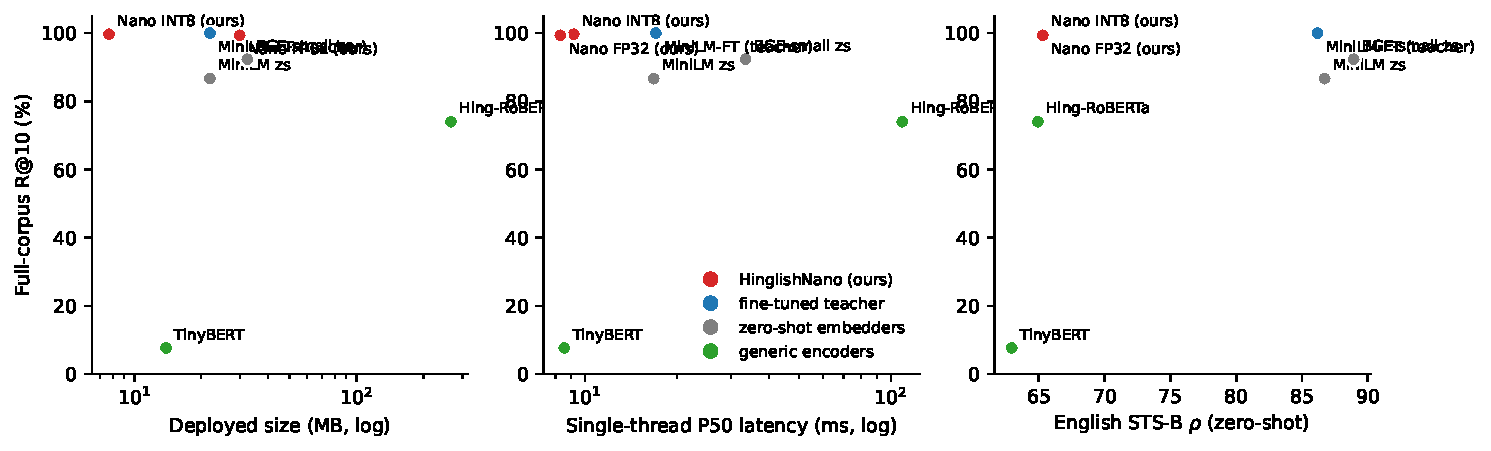
\includegraphics[width=\textwidth]{fig_frontier.pdf}
\caption{The quality--efficiency frontier. (a) Full-corpus R@10 vs.\ deployed size; (b) vs.\ single-thread latency; (c) the specialization trade-off: English STS-B vs.\ in-domain R@10. \nano{} occupies the small-fast corner without leaving the top recall tier; TinyBERT shares the corner but is not a usable embedder (R@10 7.7).}
\label{fig:frontier}
\end{figure}

\subsection{Fine-tuning schedule control}
Table~\ref{tab:budget} reports the control that this paper's comparative claims rest on. At 3 epochs the fine-tuned teacher scores 79.0 R@1 / 81.3 HardR@1 (1-vs-20) and trails \nano{} by 7 points; at 30 epochs it reaches 99.0 and leads by 7. Any comparison of a task-trained small model against a lightly fine-tuned baseline is unsound without schedule disclosure. We report all \nano{}-vs-teacher comparisons against the 30-epoch model.

\begin{table}[t]
\centering\small
\caption{Fine-tuning schedule control (1-vs-20 protocol). Reversal of the ranking between 3 and 30 fine-tuning epochs motivates mandatory schedule disclosure for baseline fine-tuning.}
\label{tab:budget}
\begin{tabular}{lrrrrr}
\toprule
System & Steps & R@1 & HardR@1 & hard margin & STS-B $\rho$ \\
\midrule
\nano{} V5 (ours, 30 ep) & 5{,}250 & 92.0 & 92.3 & $+0.175$ & 65.3 \\
MiniLM-FT, 3 epochs & 195 & 79.0 & 81.3 & $+0.106$ & 86.8 \\
MiniLM-FT, 30 epochs & 1{,}950 & 99.0 & 99.0 & $+0.439$ & 86.2 \\
\bottomrule
\end{tabular}
\end{table}

\subsection{Robustness to candidate-set scale}
Figure~\ref{fig:degradation} tracks R@1 as the candidate pool grows from 20 to 1{,}245. \nano{} degrades least ($-4.0$), the saturated teacher $-7.0$, BGE $-9.7$, zero-shot MiniLM $-15.7$, and Hing-RoBERTa $-24.3$, falling \emph{below} zero-shot MiniLM at scale. Figure~\ref{fig:margin} illustrates the underlying mechanism: degradation is correlated with the 1-vs-20 hard-negative margin (Pearson $r=0.73$ across the seven evaluated models\footnote{Exact value printed by the evaluation script; reflects margin trends across tested systems.}). Hing-RoBERTa's compressed cosine space ($+0.03$ margin) ranks gold first among few candidates but cannot survive 1{,}245; margin, not R@1 on small candidate sets, is the quantity that generalizes. This is why our protocol reports both.

\begin{figure}[t]
\centering
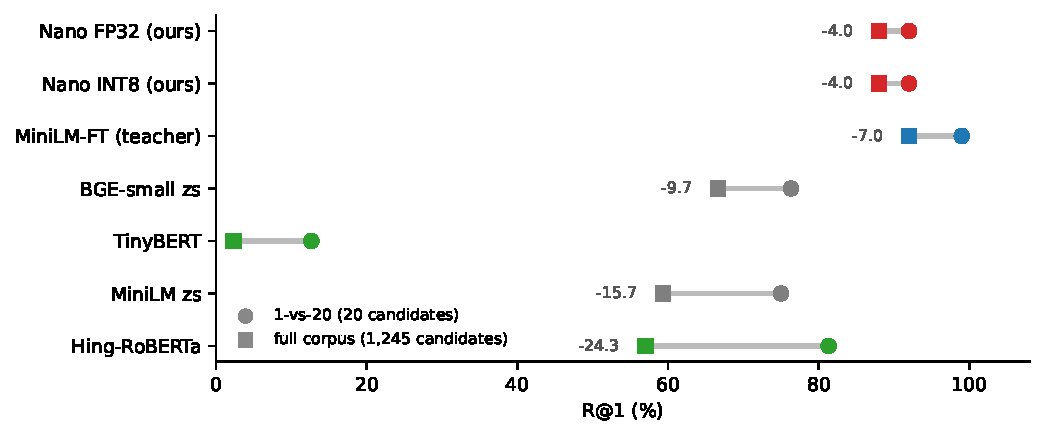
\includegraphics[width=0.78\textwidth]{fig_degradation.pdf}
\caption{R@1 under candidate-set scaling (circles: 1-vs-20; squares: full corpus). \nano{} is the most scale-robust system; Hing-RoBERTa loses 24.3 points.}
\label{fig:degradation}
\end{figure}

\begin{figure}[t]
\centering
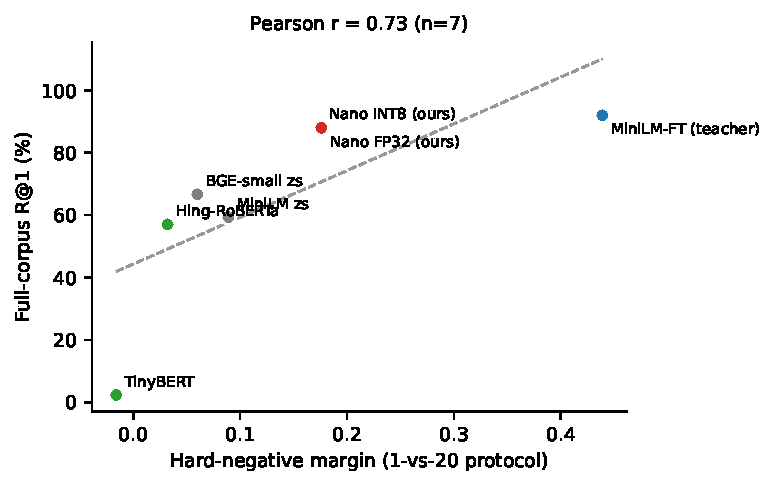
\includegraphics[width=0.5\textwidth]{fig_margin.pdf}
\caption{Hard-negative margin (small-candidate protocol) vs.\ full-corpus R@1. Margin correlates with scale robustness; systems with near-zero or negative margins collapse when the candidate pool grows.}
\label{fig:margin}
\end{figure}

\subsection{Latency and footprint}
Figure~\ref{fig:latency}. \nano{} FP32 is the fastest usable embedder measured ($P_{50}$ 8.3\,ms, 120 QPS single-thread); TinyBERT-INT8 is latency-comparable (8.6\,ms) but unusable as an embedder (R@1 2.3), so we claim \emph{fastest usable}, not fastest. \nano{} INT8 is $1.9\times$ faster than the fine-tuned teacher (9.2 vs.\ 17.0\,ms), $3.6\times$ BGE, $11.9\times$ Hing-RoBERTa. Our own dynamic INT8 is 11\% slower than our FP32 at batch 1---INT8 is the \emph{footprint} decision (7.7 vs.\ 29.8\,MB, $3.9\times$), FP32 the latency decision; both configurations are reported and quantization exhibits no measurable degradation within evaluation resolution (identical retrieval and STS-B to within one query and 0.03 $\rho$).

\begin{figure}[t]
\centering
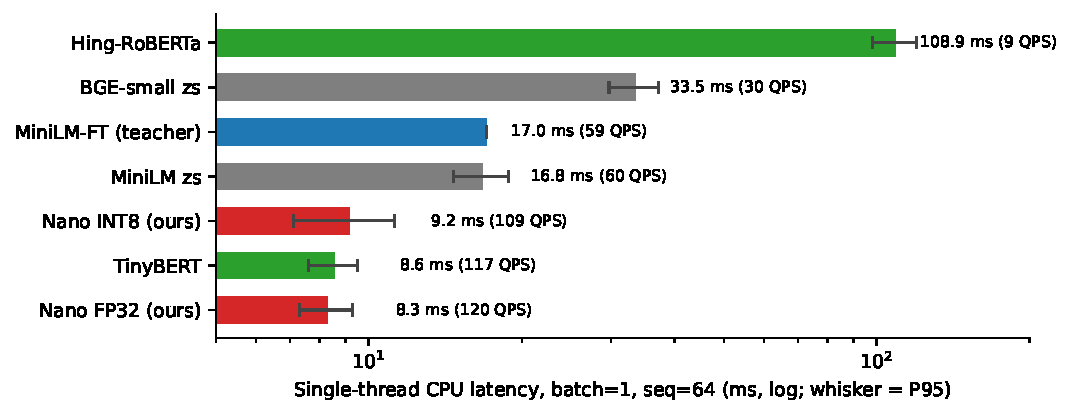
\includegraphics[width=0.8\textwidth]{fig_latency.pdf}
\caption{Single-thread CPU latency (batch 1, seq 64, tokenization excluded; whiskers = $P_{95}$). All systems INT8-ONNX except \nano{} FP32.}
\label{fig:latency}
\end{figure}

\subsection{English STS-B: the specialization trade-off}
\nano{} scores $\rho=65.3$ [62.3, 68.3], comparable to Hing-RoBERTa (64.9 [61.7, 67.9]) and TinyBERT (62.9), and $21.4$--$23.6$ points below MiniLM/BGE. This is the declared cost of a 7.77M domain-specialized student; we do not claim general-purpose embedding capability. Notably, the fine-tuned teacher \emph{retains} its English STS-B (86.2), so the in-domain gap between student and teacher is not explained by specialization damage in the teacher.

\subsection{Multi-task heads (held-out)}
\begin{table}[t]
\centering\small
\caption{Auxiliary heads on the 1{,}648-row held-out split (INT8 checkpoint). NER quality is deliberately not claimed (see text).}
\begin{tabular}{ll}
\toprule
Gate & 90.5\% acc / 93.7 F1 (P 93.9, R 93.4) \\
Chatter false-positive probe & 20.3\% [95\% CI 12.0, 32.3] ($n{=}59$) \\  % FIX 2: measured value
Domain (6-way) & 65.4\% (weakest head) \\                            % FIX 4: unfulfilled artifact claim removed
Temporal scope (3-way) & 86.7\% \\
NER (17-tag BIO) & capability claim \emph{withheld}: in-distribution span-F1 65.3 \\
 & drops to 18.5 on out-of-template data $\Rightarrow$ template-bound \\
 & deferred to LinCE \texttt{ner\_hineng} evaluation \\              % TODO(after LinCE): replace with measured F1 + coverage
\bottomrule
\end{tabular}
\end{table}

The gate performs solidly on information-bearing utterances but suppresses only 79.7\% [95\% CI 67.7, 88.0] of chatter. The false positives are not random: they concentrate on \emph{evaluative and reactive} utterances (``hilarious'', ``superb'', ``too funny'') and self-state reports (``thak gaya hu''), indicating the gate keys on affective rather than informational content. A structural cause is documented in Sec.~3.1: the 840 synthetic chatter rows fell entirely into the validation split, so the gate never trained on synthetic chatter of any kind. Domain is the weakest head (65.4\%). NER remains unclaimed pending the LinCE evaluation.

\section{Discussion}
\label{sec:discussion}
\textbf{Why the student trails at top-1.} Four mechanisms, in probable order of recoverability: (1) \emph{checkpoint selection}---the deployed model is the epoch-8 composite-best, but the contrastive loss improved for 22 further epochs; (2) \emph{signal cleanliness}---the teacher's fine-tuning used exactly the 16{,}593 rows with clean (query, positive, negatives) triplets, while 26\% of our contrastive batch was identity pairs; (3) \emph{multi-task dilution}---the embedding objective shares capacity and gradient with four classification heads via uncertainty weighting; (4) \emph{capacity} ($2.9\times$). We tested a fifth hypothesis and rejected it: the domain-native tokenizer yields only $1.24\times$ less fragmentation than MiniLM's WordPiece (18.9 vs.\ 23.4 tokens/query), far too small to explain a 4-point gap. We report this negative result because tokenizer nativeness is a common but rarely quantified justification.

\textbf{Deployment guidance.} For a memory engine whose top-$k$ feeds selection or a reranker, \nano{} INT8 is the Pareto choice: top-10 recall within one query of the saturated fine-tuned teacher, $2.8\times$ smaller, $1.9\times$ faster, and four decisions for free. When exact top-1 autonomous matching is required and 22\,MB is affordable, the fine-tuned teacher remains better. INT8 vs.\ FP32 is a size-vs-latency decision, not a quality one.

\section{Limitations}
(1) $n{=}300$ test queries caps detectable differences at $\approx$2 points. (2) The store contains 1{,}245 memories; behavior at $10^4$--$10^5$ candidates is untested, though the margin analysis suggests ordering is preserved. (3) Latency is measured on one CPU (Xeon @2.0\,GHz, 2 cores); other hardware may reorder the INT8/FP32 trade-off. (4) Single training seed; inference-side CIs are reported but not training-seed variance. % TODO(optional, after seed retrains): add mean±std and reword
(5) The domain head is weak (65.4\%) and the gate misclassifies evaluative chatter (Sec.~5.6). (6) NER is unevaluated on public benchmarks and prior evidence indicates template sensitivity. % TODO(after LinCE): update with measured numbers
(7) The corpus is proprietary; the held-out test split, scripts, and per-query results are released to mitigate but not eliminate this.

\section{Conclusion and Future Work}
\nano{}-V5 demonstrates that a sub-8\,MB multi-task encoder can achieve high retrieval fidelity---top-10 recall statistically comparable with a fine-tuned teacher $2.9\times$ its size---while paying a quantified, disclosed price in top-1 precision and general-purpose STS. Future work, in order of expected payoff: checkpoint selection by held-out retrieval metric rather than composite score; filtering identity-positive pairs from the contrastive loss; consuming both curated hard negatives; moving the chatter augmentation into the training split and extending it with evaluative and reactive utterances; trimming the embedding vocabulary; LinCE \texttt{ner\_hineng} evaluation; and store-scale testing beyond $10^4$ candidates.

\section*{Reproducibility}
Environment: Intel Xeon @2.0\,GHz (2 physical cores), 33.7\,GB RAM; Python 3.12.13, PyTorch 2.10.0, ONNX Runtime 1.30.0; all inference single-thread (torch and ORT pinned). We release: the 300-query test set with golds and the 1{,}245-memory candidate store; the full benchmark suite (both retrieval protocols, STS-B, latency, paired statistics); per-query rankings (\texttt{benchmark\_results\_v3.json}); figure-generation scripts; and the model artifacts at \url{https://github.com/unshakensoul17/HinglishNano_Reserach_paper} and Hugging Face Hub at \url{https://huggingface.co/unsahkensoul18/Hinglishnano_V5}.
\begin{thebibliography}{20}\small
\bibitem{reimers2019} N. Reimers and I. Gurevych. \emph{Sentence-BERT: Sentence Embeddings using Siamese BERT-Networks.} EMNLP 2019.
\bibitem{wang2020} W. Wang, F. Wei, L. Dong, H. Bao, N. Yang, M. Zhou. \emph{MiniLM: Deep Self-Attention Distillation for Task-Agnostic Compression of Pre-Trained Transformers.} NeurIPS 2020.
\bibitem{xiao2023} S. Xiao, Z. Liu, P. Zhang, N. Muennighoff, D. Xiong, C. Lin. \emph{C-Pack: Packaged Resources To Advance General Chinese Embedding.} arXiv:2309.07597, 2023.
\bibitem{nagireddy2023} S. Nagireddy et al. \emph{L3Cube-HingCorpus and HingBERT: A Code-Mixed Hindi--English Dataset and Transformer Models.} arXiv:2204.08398, 2023.
\bibitem{aguilar2020} G. Aguilar, F. Dalvi, S. Kar, et al. \emph{LinCE: A Centralized Benchmark for Linguistic Code-Switching Evaluation.} LREC 2020.
\bibitem{muennighoff2023} N. Muennighoff et al. \emph{MTEB: Massive Text Embedding Benchmark.} EACL 2023.
\bibitem{thakur2021} N. Thakur, N. Reimers, A. R\"uckle, et al. \emph{BEIR: A Heterogeneous Benchmark for Zero-shot Evaluation of Information Retrieval Models.} NeurIPS Datasets and Benchmarks 2021.
\bibitem{jiao2020} X. Jiao et al. \emph{TinyBERT: Distilling BERT for Natural Language Understanding.} ICLR 2020.
\bibitem{hinton2015} G. Hinton, O. Vinyals, J. Dean. \emph{Distilling the Knowledge in a Neural Network.} arXiv:1503.02531, 2015.
\bibitem{henderson2017} M. Henderson et al. \emph{Efficient Natural Language Response Suggestion for Smart Reply.} arXiv:1705.00652, 2017.   % FIX 7: garbled author name removed
\bibitem{ainslie2023} J. Ainslie et al. \emph{GQA: Training Generalized Multi-Query Transformer Models from Multi-Head Checkpoints.} EMNLP 2023.
\bibitem{su2021} J. Su et al. \emph{RoFormer: Enhanced Transformer with Rotary Position Embedding.} arXiv:2104.09864, 2021.
\bibitem{shazeer2020} N. Shazeer. \emph{GLU Variants Improve Transformer.} arXiv:2002.05202, 2020.
\bibitem{zhang2019} B. Zhang, R. Sennrich. \emph{Root Mean Square Layer Normalization.} NeurIPS 2019.
\bibitem{jacob2018} B. Jacob et al. \emph{Quantization and Training of Neural Networks for Efficient Integer-Arithmetic-Only Inference.} CVPR 2018.
\bibitem{wang2018glue} A. Wang et al. \emph{GLUE: A Multi-Task Benchmark and Analysis Platform for Understanding Natural Language.} NeurIPS 2018.
\bibitem{conneau2020} A. Conneau et al. \emph{Unsupervised Cross-lingual Representation Learning at Scale.} ACL 2020.
\end{thebibliography}

\appendix
\section{1-vs-20 protocol (secondary results)}
\begin{table}[h]
\centering\small
\caption{1-vs-20 protocol: 20 candidates = gold + curated hard negatives ($\le2$) + seeded corpus distractors. Saturates for strong systems (R@3 $\ge 90.7$). 95\% bootstrap CIs in brackets.}
\begin{tabular}{lrrrrr}
\toprule
Model & R@1 & R@3 & MRR@10 & HardR@1 & margin \\
\midrule
\nano{} V5 INT8 & 92.0 {\tiny[88.7,95.0]} & 100.0 & 95.7 & 92.3 {\tiny[89.0,95.3]} & $+0.175$ \\
\nano{} V5 FP32 & 92.0 {\tiny[88.7,95.0]} & 100.0 & 95.7 & 92.3 {\tiny[89.0,95.3]} & $+0.176$ \\
MiniLM (zs) & 75.0 {\tiny[69.7,80.0]} & 97.0 & 85.2 & 79.3 {\tiny[74.7,84.0]} & $+0.089$ \\
BGE-small (zs) & 76.3 {\tiny[71.7,81.0]} & 98.3 & 86.9 & 78.7 {\tiny[74.0,83.3]} & $+0.060$ \\
Hing-RoBERTa & 81.3 {\tiny[77.0,85.7]} & 90.7 & 86.6 & 93.7 {\tiny[90.7,96.3]} & $+0.032$ \\
TinyBERT-4L & 12.7 {\tiny[9.0,16.7]} & 33.7 & 28.5 & 36.3 {\tiny[31.0,42.0]} & $-0.016$ \\
MiniLM-FT (30ep) & 99.0 {\tiny[97.7,100.0]} & 99.0 & 99.5 & 99.0 {\tiny[97.7,100.0]} & $+0.439$ \\
\bottomrule
\end{tabular}
\end{table}

\section{Integrity checks}
The exported graph was verified to consume its attention mask (max embedding deviation $2.2\times10^{-1}$ when the mask is forced to all-ones on padded input); ONNX exports of baselines match PyTorch outputs to $3.3\times10^{-6}$; nine adversarial inputs (empty, whitespace, emoji-only, 300-character, code snippets, punctuation-only) produce valid output shapes with zero crashes; the dataset row count is asserted equal to the training-time count (24{,}039) before any split logic executes, guarding against silent split contamination.

\end{document}
